\section{Parche de Misión}

El parche de misión de \textbf{PDA STARS} representa la identidad científica, la disciplina ingenieril y el espíritu de innovación del semillero aeroespacial de la Institución Educativa José Antonio Galán (La Estrella, Antioquia) en el Concurso Colombiano de Cohetería Deportiva 2026.

\begin{figure}[H]
\centering
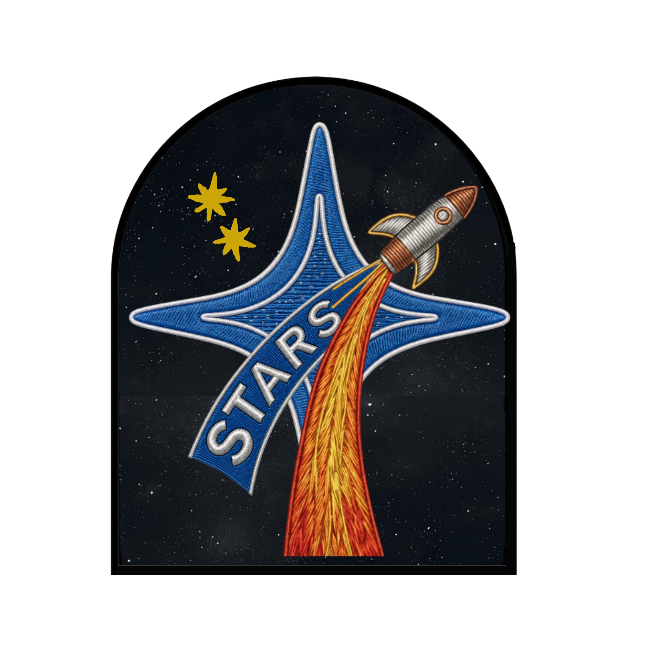
\includegraphics[width=0.42\linewidth]{parche_mision.png}
\caption{Parche oficial de la misión PDA STARS (Equipo 211).}
\label{fig:parche_mision}
\end{figure}

\subsection{Significado y Simbolismo Técnico}
\begin{itemize}[leftmargin=1.5em]
    \item \textbf{El Cohete en Ascenso:} Simboliza el desarrollo estructural, la propulsión eficiente con el motor oficial Estes F15-4 y la precisión requerida para alcanzar el apogeo reglamentario de 300 metros con trayectoria vertical estable.
    \item \textbf{Las Estrellas:} Rinden tributo al municipio de La Estrella (cuna del equipo) y a las metas de excelencia científica trazadas por los estudiantes galanistas.
    \item \textbf{La Órbita y Estela:} Representan la integración interdisciplinaria entre la física atmosférica, la simulación computacional de vuelo, la instrumentación electrónica de la carga útil y la recuperación segura.
    \item \textbf{La Paleta Cromática:} El azul institucional refleja la serenidad y rigor analítico; el dorado evoca la calidad y perseverancia en las pruebas experimentales; el rojo personifica la energía de la combustión del grano sólido y la pasión investigativa.
\end{itemize}
